\documentclass{article}
\usepackage{tikz}
\usetikzlibrary{calc}
\usetikzlibrary{shapes.geometric, arrows, positioning}
\usepackage{amsmath}

\title{Social Predict - Weighted Probability Adjustment Model (WPAM) for Market Pricing and Divergence-Based Payout Model (DBPM) for Payout Distributions}
\author{Patrick Delaney}
\date{November 2024}

% Define the macro to draw pie charts
\newcommand{\piechart}[3]{ % #1: x-coordinate, #2: y-coordinate, #3: fraction (0 to 1)
  \draw (#1,#2) circle (0.5); % Draw circle at (#1,#2) with radius 0.5
  \pgfmathsetmacro{\startangle}{90}
  \pgfmathsetmacro{\endangle}{90 - 360 * #3} % Calculate end angle based on fraction
  \filldraw[fill=cyan!50] (#1,#2) -- ++(\startangle:0.5) arc (\startangle:\endangle:0.5) -- cycle; % Draw filled sector
}

\begin{document}

\maketitle

\section{Overview}

\begin{itemize}
    \item \textbf{Overall Purpose:} The purpose of this document is to describe in clear detail with graphical illustrations how market pricing (probability) gets set and how points/money/units gets distributed from a series of historical bets/transactions.
    \item \textbf{Ab Initio:} Since our software is stateless, the market price and how a pool of points gets distributed should be able to be calculated from the starting point of a string of transactions. There is no need to cache or store calculations along the way.
    \item \textbf{Transparency and Unit Testing:} Given that pricing and distribution is fundamental to how the software works, it is essential to ensure the full algorithm is well understood in order to write proper unit tests and to communicate the rules to users and participants.
\end{itemize}

\section{Conventions}

\begin{itemize}
    \item \textbf{Course Payouts Divide By Zero Condition:} When Course Payouts calculations and further calculations derived from Course Payouts may include an inf (divide by zero) condition, we will define the output as zero. This situation arises in which the Market Value is measured as zero, since everyone has exited the market. Technically the market Value is still equal to the initial investment value until the resolution has been fulfilled, so the Course Payouts, which simply represent a link between the probability and the payout at a given market condition, are not representative of the final state of the market. Thus, calling the Course Payouts and anything calculated from the Course Payouts zero makes sense.
\end{itemize}

\section{Positions Flow Cart}

\begin{itemize}
    \item \textbf{Exchange, Transform, Load:} The net positions that every trader has on any given market are calculated through what is basically an Exchange, Transform and Load (ETL) pipeline. We Exchange the data in the form of transactions, Transform it through a series of steps as shown in the chart below, and finally we Load the net positions as an object.
    \item \textbf{Works Anytime:} The ETL pipeline shown in the chart works at any point in the market's history, including after the resolution. Positions could be calculated for a market resolution at ay given percentage between 0 pc and 100 pc or at 0 (NO) or 100 (YES) pc resolutions.
\end{itemize}


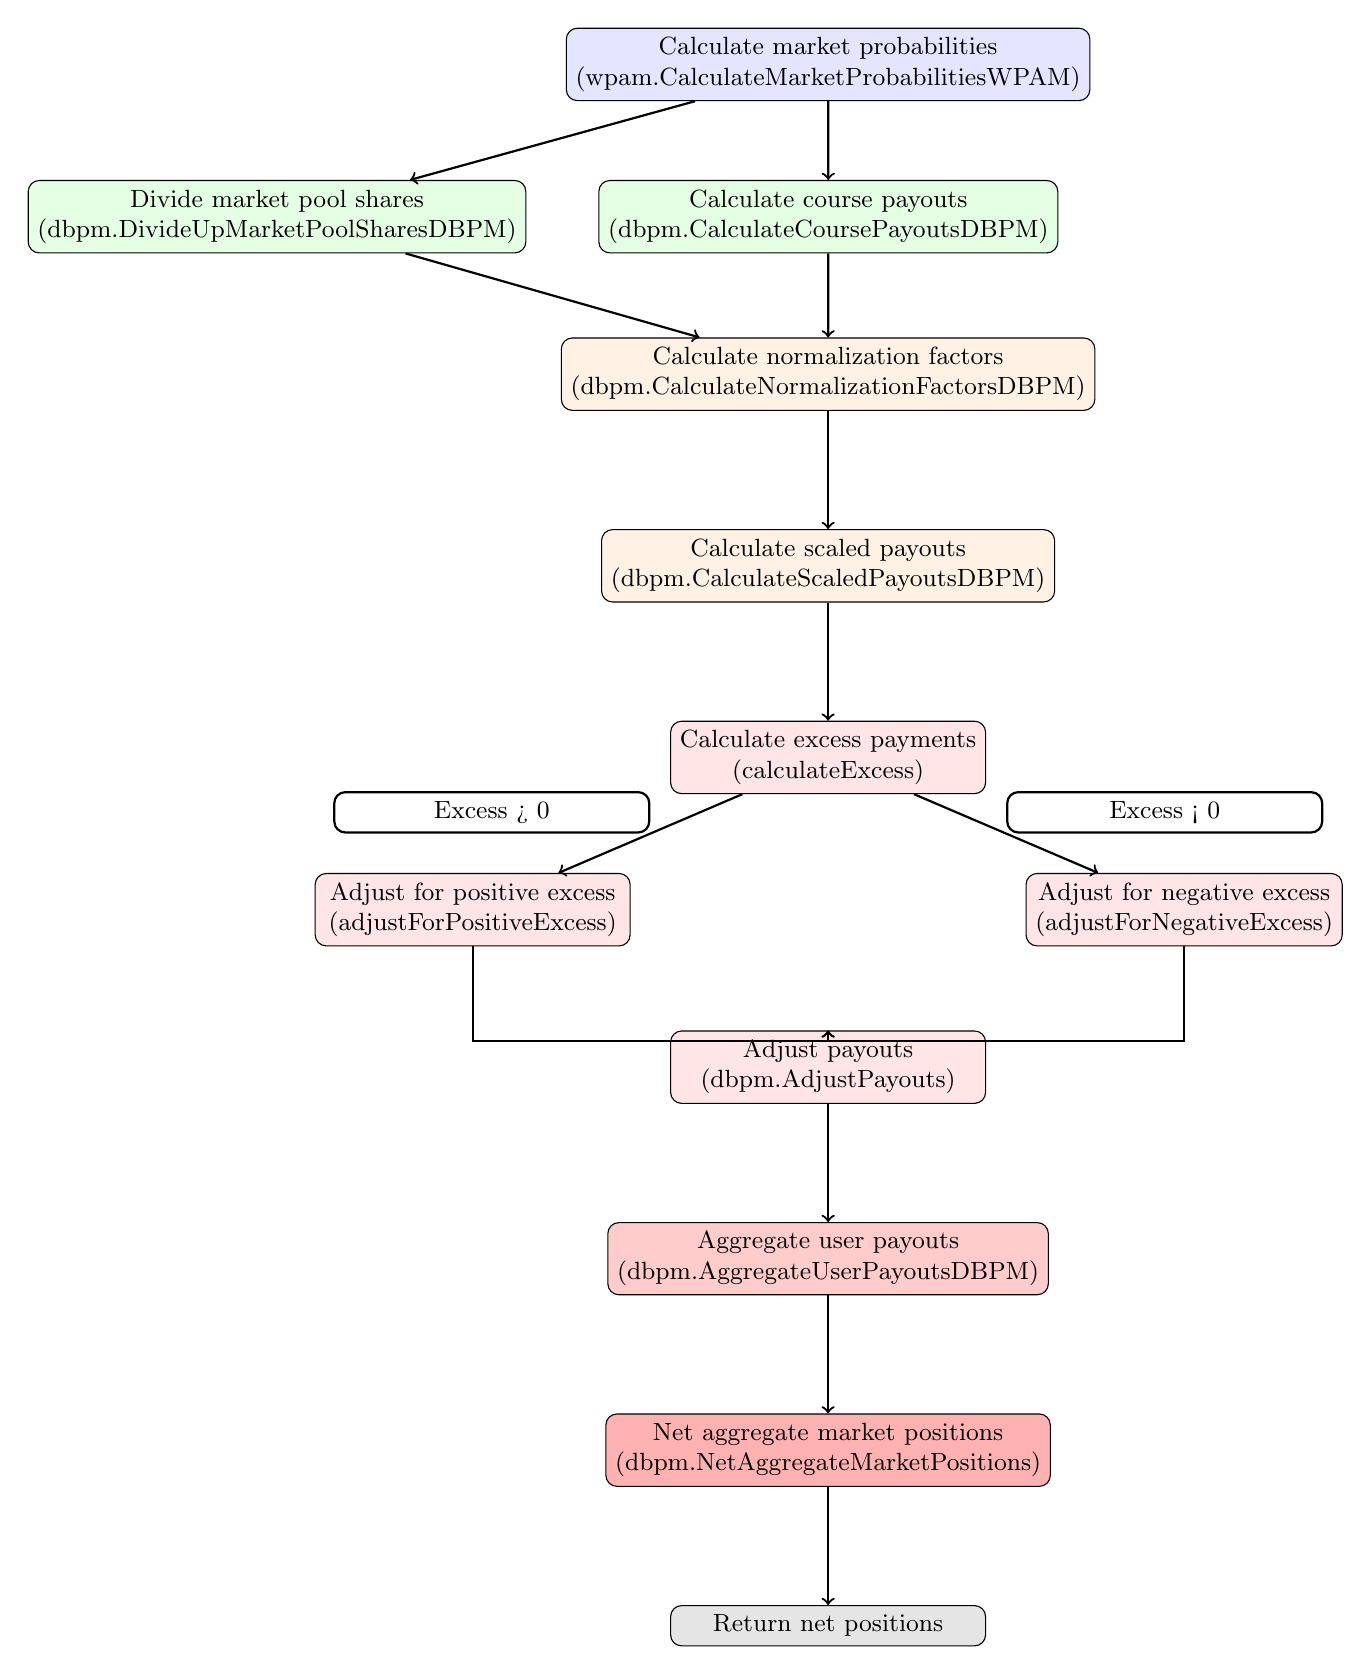
\begin{tikzpicture}[
    node distance=1.5cm,
    every node/.style={rectangle, rounded corners, draw=black, align=center, font=\small, minimum width=4cm},
    arrow/.style={->, thick}
]

% Nodes
\node (calcProbs) [fill=blue!10] {Calculate market probabilities \\ (wpam.CalculateMarketProbabilitiesWPAM)};

% Parallel nodes: Divide Shares and Course Payouts, placed closer together
\node (divideShares) [below left=1cm and 0.5cm of calcProbs, fill=green!10] {Divide market pool shares \\ (dbpm.DivideUpMarketPoolSharesDBPM)};
\node (coursePayouts) [below right=1cm and -6.25cm of calcProbs, fill=green!10] {Calculate course payouts \\ (dbpm.CalculateCoursePayoutsDBPM)};

% Next node: Normalization Factors
\node (normFactors) [below=3cm of calcProbs, fill=orange!10] {Calculate normalization factors \\ (dbpm.CalculateNormalizationFactorsDBPM)};

% Scaled Payouts
\node (scaledPayouts) [below=of normFactors, fill=orange!10] {Calculate scaled payouts \\ (dbpm.CalculateScaledPayoutsDBPM)};

% Adjust Payouts Nodes
\node (calculateExcess) [below=of scaledPayouts, fill=red!10] {Calculate excess payments \\ (calculateExcess)};
\node (adjustPosExcess) [below left=1cm and 0.5cm of calculateExcess, fill=red!10] {Adjust for positive excess \\ (adjustForPositiveExcess)};
\node (adjustNegExcess) [below right=1cm and 0.5cm of calculateExcess, fill=red!10] {Adjust for negative excess \\ (adjustForNegativeExcess)};
\node (adjustPayouts) [below=3cm of calculateExcess, fill=red!10] {Adjust payouts \\ (dbpm.AdjustPayouts)};

% Aggregation and Final Steps
\node (aggregatePayouts) [below=of adjustPayouts, fill=red!20] {Aggregate user payouts \\ (dbpm.AggregateUserPayoutsDBPM)};
\node (netPositions) [below=of aggregatePayouts, fill=red!30] {Net aggregate market positions \\ (dbpm.NetAggregateMarketPositions)};
\node (end) [below=of netPositions, fill=gray!20] {Return net positions};

% Arrows
\draw[arrow] (calcProbs) -- (divideShares);
\draw[arrow] (calcProbs) -- (coursePayouts);
\draw[arrow] (divideShares) -- (normFactors);
\draw[arrow] (coursePayouts) -- (normFactors);
\draw[arrow] (normFactors) -- (scaledPayouts);
\draw[arrow] (scaledPayouts) -- (calculateExcess);
\draw[arrow] (calculateExcess) -- (adjustPosExcess) node[midway, above left] {Excess > 0};
\draw[arrow] (calculateExcess) -- (adjustNegExcess) node[midway, above right] {Excess < 0};
\draw[arrow] (adjustPosExcess.south) -- ++(0,-1.2) -| (adjustPayouts.north);
\draw[arrow] (adjustNegExcess.south) -- ++(0,-1.2) -| (adjustPayouts.north);
\draw[arrow] (adjustPayouts) -- (aggregatePayouts);
\draw[arrow] (aggregatePayouts) -- (netPositions);
\draw[arrow] (netPositions) -- (end);

\end{tikzpicture}


\newpage

\section{First Transaction}

\begin{itemize}
    \item \textbf{Initial Investment:} Every market is assumed to have an initial investment of at least 1. This investment comes from a fee assessed to the market creator. This initial investment goes both in the numerator and denominator of the probability calculation.
    \item \textbf{Initial Probability:} Every market starts out at a probability of 0.5 which means even odds between a YES and NO outcome.
    \item \textbf{First Transaction:} In our sample below, the first transaction is a bet of 20 Units in the NO direction.
\end{itemize}

\begin{center}

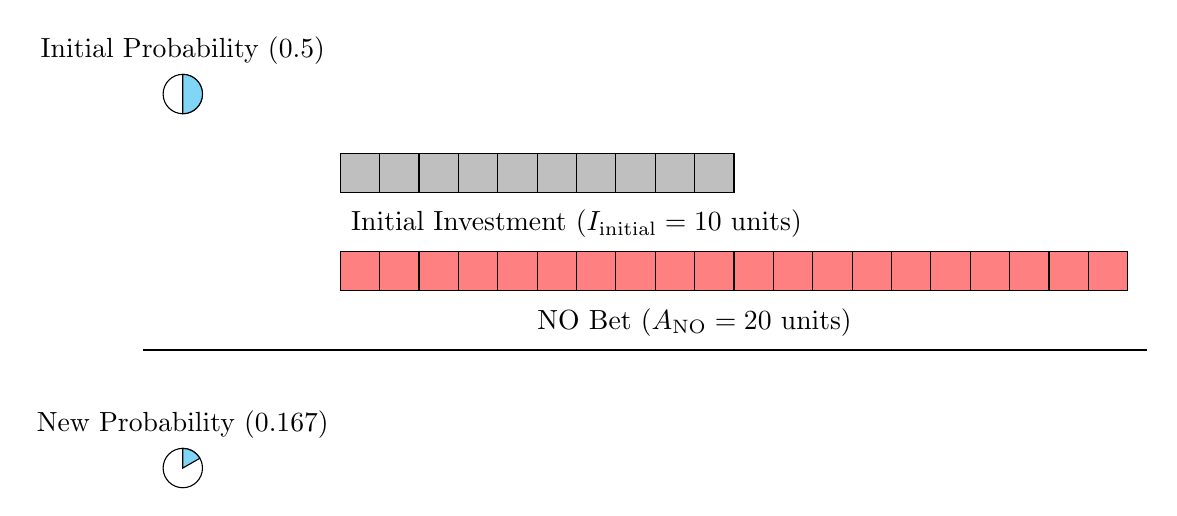
\begin{tikzpicture}[scale=0.5]

% Pie Chart for Initial Probability 0.5 at x = -1, y = 2.5
\piechart{-1}{2.5}{0.5}
\node[above] at (-1,3) {Initial Probability (0.5)};

% Pie Chart for New Probability 0.167 at x = -1, y = -7
\piechart{-1}{-7}{0.167}
\node[above] at (-1,-6.5) {New Probability (0.167)};

% Initial Investment (Gray Squares)
\foreach \x in {3,...,12}
{
    \draw[fill=gray!50] (\x,0) rectangle ++(1,1);
}

% NO Bet (Red Squares), set down by -2.5
\foreach \x in {3,...,22}
{
    \draw[fill=red!50] (\x,-2.5) rectangle ++(1,1);
}

% Horizontal Line between the transaction block and updated probability
\draw[thick] (-2,-4.0) -- (23.5,-4.0);

% Labels
\node[below] at (9,-0.2) {Initial Investment (\(I_{\text{initial}} = 10\) units)};
\node[below] at (12,-2.7) {NO Bet (\(A_{\text{NO}} = 20\) units)};

\end{tikzpicture}
\end{center}

\[
P_{\text{new}} = \frac{P_{\text{initial}} \times I_{\text{initial}} + A_{\text{YES}}}{I_{\text{initial}} + A_{\text{YES}} + A_{\text{NO}}} = \frac{0.5 \times 10 + 0}{10 + 0 + 20} = \frac{5}{30} \approx 0.167
\]

% **Add the market share division calculations here**

\subsection*{Market Share Division}

\begin{itemize}
    \item \textbf{Banker's Rounded Share Pool:} First we look at how many total shares of YES and NO exist in the market pool as a whole by using the WPAM. The total share pool is equal to the Total Market Volume, not including the initial investment. The total share pool times the Probability will be the YES shares, while 1-(Probability) times the total share pool will be the NO shares.
    \item  \textbf{Recuperating Initial Investment:} The initial investment paid in by the market maker can be recuperated at the end after the resolution has been made. In effect, the initial market investment is held in escrow in exchange for a fee by the computer. After the resolution, the market maker bonus can be paid out and the initial investment will be redistributed to all market participants.
\end{itemize}

\[
S = \text{Total Market Volume} = 20 \text{ units}
\]


\begin{align*}
S_{\text{YES}} &= \left\lfloor S \times P_{\text{new}} \right\rceil = \left\lfloor 20 \times 0.167 \right\rceil = 3 \\
S_{\text{NO}} &= \left\lfloor S \times (1 - P_{\text{new}}) \right\rceil = \left\lfloor 20 \times 0.833 \right\rceil = 17
\end{align*}


\begin{center}
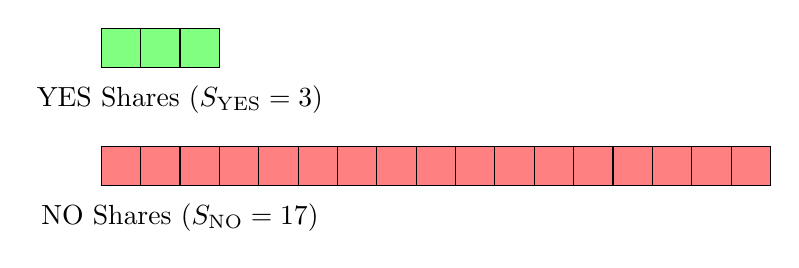
\begin{tikzpicture}[scale=0.5]

% YES Shares (Green Squares), set down by -6
\foreach \x in {1,...,3}
{
    \draw[fill=green!50] (\x,-6) rectangle ++(1,1);
}

% NO Shares (Red Squares), set down by -6
\foreach \x in {1,...,17}
{
    \draw[fill=red!50] (\x,-9) rectangle ++(1,1);
}

% Labels
\node[below] at (3,-6.2) {YES Shares (\(S_{\text{YES}} = 3\))};
\node[below] at (3,-9.2) {NO Shares (\(S_{\text{NO}} = 17\))};

\end{tikzpicture}
\end{center}

% Double Divider Line To Next Step
\begin{center}
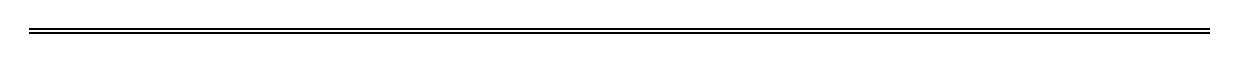
\begin{tikzpicture}[scale=0.5]
\draw[thick] (0,-1) -- (30,-1);
\draw[thick] (0,-1.1) -- (30,-1.1);
\end{tikzpicture}
\end{center}

\newpage

\section{Second Transaction}

\begin{itemize}
    \item \textbf{Second Transaction:} A different bettor comes in and places 10 units in the YES direction.
\end{itemize}

\begin{center}
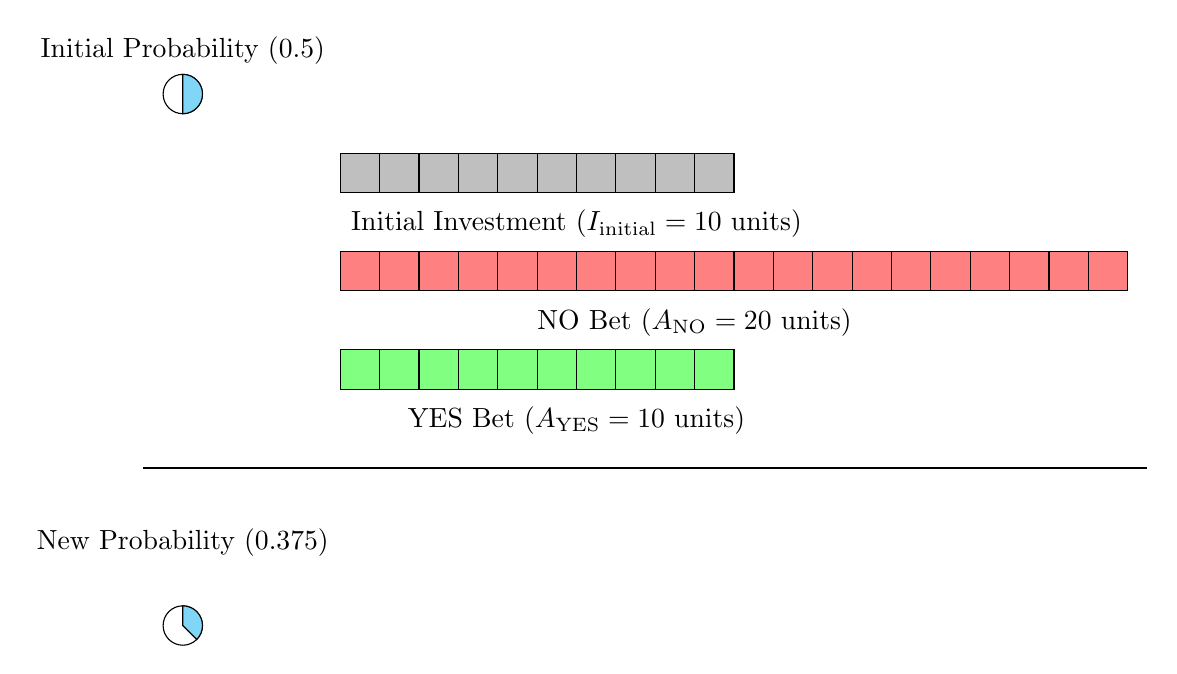
\begin{tikzpicture}[scale=0.5]

% Pie Chart for Initial Probability 0.5 at x = -1, y = 2.5
\piechart{-1}{2.5}{0.5}
\node[above] at (-1,3) {Initial Probability (0.5)};

% Pie Chart for New Probability 0.375 at x = -1, y = -7
\piechart{-1}{-11}{0.375}
\node[above] at (-1,-9.5) {New Probability (0.375)};

% Initial Investment (Gray Squares)
\foreach \x in {3,...,12}
{
    \draw[fill=gray!50] (\x,0) rectangle ++(1,1);
}

% YES Bet (Green Squares)
\foreach \x in {3,...,12}
{
    \draw[fill=green!50] (\x,-5) rectangle ++(1,1);
}

% NO Bet (Red Squares)
\foreach \x in {3,...,22}
{
    \draw[fill=red!50] (\x,-2.5) rectangle ++(1,1);
}

% Horizontal Line between the squares
\draw[thick] (-2,-7.0) -- (23.5,-7.0);

% Labels
\node[below] at (9,-0.2) {Initial Investment (\(I_{\text{initial}} = 10\) units)};
\node[below] at (12,-2.7) {NO Bet (\(A_{\text{NO}} = 20\) units)};
\node[below] at (9,-5.2) {YES Bet (\(A_{\text{YES}} = 10\) units)};

\end{tikzpicture}
\end{center}

\[
P_{\text{new}} = \frac{0.5 \times 10 + 10}{10 + 10 + 20} = \frac{15}{40} \approx 0.375
\]

\subsection*{Market Share Division}

\[
S = \text{Total Market Volume} + I_{\text{initial}} = (10 + 20) = 30 \text{ units}
\]

\begin{align*}
S_{\text{YES}} &= \left\lfloor S \times P_{\text{new}} \right\rceil = \left\lfloor 30 \times 0.375 \right\rceil = 11 \\
S_{\text{NO}} &= \left\lfloor S \times (1 - P_{\text{new}}) \right\rceil = \left\lfloor 30 \times 0.625 \right\rceil = 19
\end{align*}

\begin{center}
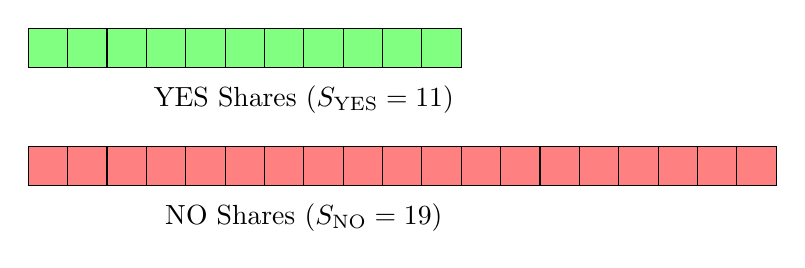
\begin{tikzpicture}[scale=0.5]

% YES Shares (Green Squares), set down by -9
\foreach \x in {1,...,11}
{
    \draw[fill=green!50] (\x,-9) rectangle ++(1,1);
}

% NO Shares (Red Squares), set down by -9
\foreach \x in {1,...,19}
{
    \draw[fill=red!50] (\x,-12) rectangle ++(1,1);
}

% Labels
\node[below] at (8,-9.2) {YES Shares (\(S_{\text{YES}} = 11\))};
\node[below] at (8,-12.2) {NO Shares (\(S_{\text{NO}} = 19\))};

\end{tikzpicture}
\end{center}

% Double Divider Line To Next Step
\begin{center}
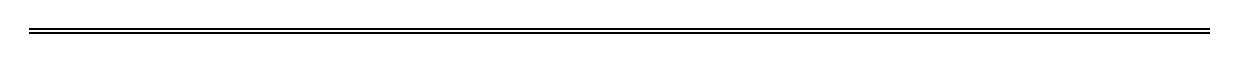
\begin{tikzpicture}[scale=0.5]
\draw[thick] (0,-1) -- (30,-1);
\draw[thick] (0,-1.1) -- (30,-1.1);
\end{tikzpicture}
\end{center}


% Single Divider Line
\begin{center}
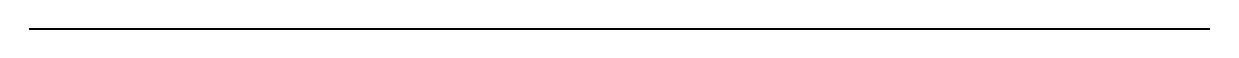
\begin{tikzpicture}[scale=0.5]
\draw[thick] (0,-1) -- (30,-1);
\end{tikzpicture}
\end{center}

% New Section: Calculating Course Payouts

\section*{Calculating Course Payouts}

\begin{itemize}
    \item \textbf{Course Payouts:} The purpose of the Course Payouts is to create a relationship between the probability, which is a float, rational positive numbers, and shares, which are of type int64, integers. We use a linear weight for each historical bet in the history of the market to create a reward factor.
    \item \textbf{Reward Factor:} Course payouts are calculated in two steps, first by calculating a reward factor \(d_i\), which is the distance from the current probability of the market \(R\), and the probability at which the bet was made \(p_i\).
    \item \textbf{New Probability After Bet, Not Previous Probability:} The current probability on the market, \(R\) is the New Probability which was just calculated by our WPAM function, \(wpam.CalculateMarketProbabilitiesWPAM\) given the bet that was just immediately made. This enforces the idea that there is no reward for simply moving the market oneself and then selling at a new probability created from that movement. In order to profit, someone else must come in and move the market further in one's favor to be able to sell.
\end{itemize}

\subsection*{Step One: Calculate Reward Factor for Each Bet}

\[
d_i = |R - p_i|
\]

\subsection*{Step Two: Calculate Course Payout for Each Bet}

\[
C_i = d_i \times b_i
\]

\subsection*{Example Calculations}

\textbf{Given:}

\begin{itemize}
  \item Resolution Probability: \( R = 0.375 \)
  \item Bet 0: Neutral, \( b_0 = 10 \) units, \( p_0 = 0.5 \)
  \item Bet 1: NO, \( b_1 = 20 \) units, \( p_1 = 0.167 \)
  \item Bet 2: YES, \( b_2 = 10 \) units, \( p_2 = 0.375 \)
\end{itemize}

\textbf{For Bet 1:}

\begin{align*}
d_1 &= |R - p_1| = |0.375 - 0.167| = 0.208 \\
C_1 &= d_1 \times b_1 = 0.208 \times 20 = 4.160 \text{ units}
\end{align*}

\textbf{For Bet 2:}

\begin{align*}
d_2 &= |R - p_2| = |0.375 - 0.375| = 0 \\
C_2 &= d_2 \times b_2 = 0 \times 10 = 0 \text{ units}
\end{align*}

% Diagram Representing Bets and Payouts in Two Columns

\begin{center}
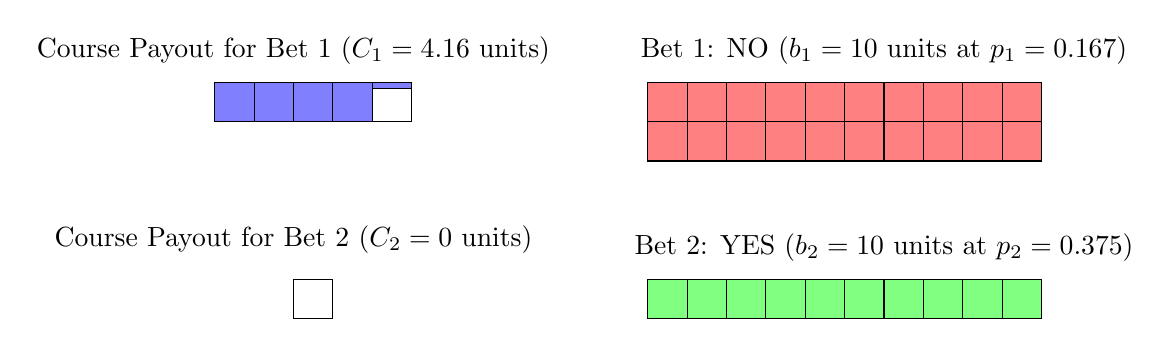
\begin{tikzpicture}[scale=0.5]

% --- Bets and Payouts for Bet 1 ---

% Bet 1: NO Bet (Red Squares), starting at x = 5
\foreach \x in {5,...,14}
{
    \draw[fill=red!50] (\x,0) rectangle ++(1,1);
    \draw[fill=red!50] (\x,-1) rectangle ++(1,1);
}

% Label for Bet 1
\node[above] at (11,1.2) {Bet 1: NO (\( b_1 = 10 \) units at \( p_1 = 0.167 \))};

% Course Payout for Bet 1 (Blue Squares), to the left of Bet 1
% Draw 3 full blue squares starting at x = 1
\foreach \x in {-6,...,-3}
{
    \draw (\x,0) rectangle ++(1,1);
    \filldraw[fill=blue!50] (\x,0) rectangle ++(1,1);
}

% Draw the partial square for 0.16 unit at x = 4
\def\xPartial{-2}  % Position of the partial square
\draw (\xPartial,0) rectangle ++(1,1);
% Fill the top 33% of the square
\filldraw[fill=blue!50] (\xPartial,0.84) rectangle ++(1,0.16);

% Label for Course Payout of Bet 1
\node[above] at (-4,1.2) {Course Payout for Bet 1 (\( C_1 = 4.16 \) units)};

% --- Bets and Payouts for Bet 2 ---

% Bet 2: NO Bet (Red Squares), starting at x = 5, y = -5
\foreach \x in {5,...,14}
{
    \draw[fill=green!50] (\x,-5) rectangle ++(1,1);
}

% Label for Bet 2
\node[above] at (11,-3.8) {Bet 2: YES (\( b_2 = 10 \) units at \( p_2 = 0.375 \))};

% Course Payout for Bet 2
% Since payout is zero, we can represent it with a zero or an empty square
\def\xPartial{-4}  % Position of the partial square
\draw (\xPartial,-5) rectangle ++(1,1);
\node at (-4,-3) {Course Payout for Bet 2 (\( C_2 = 0 \) units)};

\end{tikzpicture}
\end{center}

\section*{Normalization Factor Calculation}

The normalization factor ensures that course payouts are proportional to the total shares for each outcome, making sure that payouts align with the available market pool.

\begin{itemize}
    \item The normalization factor \( F_{\text{YES}} \) and \( F_{\text{NO}} \) adjusts each outcome's payouts so that they fit within the total shares allocated for each outcome.
    \item This prevents payouts from exceeding the total market pool, ensuring fair distribution based on the market's share allocation.
    \item By scaling payouts, the normalization factor maintains balance between YES and NO outcomes, reflecting the distribution of bets and probabilities in the market.
\end{itemize}

\newpage

\subsection*{Step Three: Calculate Normalization Factor}

\begin{itemize}
    \item At this point the normalization factor will weight everything toward NO because there are zero course payouts for YES.
\end{itemize}

Given:
\begin{itemize}
    \item Total YES Shares: \( S_{\text{YES}} = 11 \)
    \item Total NO Shares: \( S_{\text{NO}} = 19 \)
    \item Course Payouts:
    \begin{itemize}
        \item \( C_{\text{NO,1}} = 4.16 \) units
        \item \( C_{\text{YES,2}} = 0 \) units
        \item Total payout sums: \( C_{\text{YES\_SUM}} = 0 \), \( C_{\text{NO\_SUM}} = 4.16 \)
    \end{itemize}
\end{itemize}

\subsubsection*{Calculate YES Normalization Factor}

\[
F_{\text{YES}} =
\begin{cases}
      \frac{S_{\text{YES}}}{C_{\text{YES\_SUM}}} & \text{if } C_{\text{YES\_SUM}} > 0 \\
      0 & \text{if } C_{\text{YES\_SUM}} = 0
   \end{cases}
\]

Since \( C_{\text{YES\_SUM}} = 0 \), we have:

\[
F_{\text{YES}} = 0
\]

\subsubsection*{Calculate NO Normalization Factor}

\[
F_{\text{NO}} =
\begin{cases}
      \frac{S_{\text{NO}}}{C_{\text{NO\_SUM}}} & \text{if } C_{\text{NO\_SUM}} > 0 \\
      0 & \text{if } C_{\text{NO\_SUM}} = 0
   \end{cases}
\]

Since \( C_{\text{NO\_SUM}} = 4.16 \), we have:

\[
F_{\text{NO}} = \frac{19}{4.16} \approx 4.56
\]

Thus, the normalization factors are:

\[
F_{\text{YES}} = 0, \quad F_{\text{NO}} \approx 4.56
\]

\newpage


\section*{Scaled Payout Calculation for Second Transaction}

\begin{itemize}
    \item \textbf{Purpose of Scaled Payouts:}
    \begin{itemize}
        \item Scaled payouts use normalization factors to adjust the raw course payouts, ensuring they align proportionally with the total market shares for each outcome.
        \item This prevents over-distribution of payouts and ensures fairness in the final allocations.
        \item By scaling payouts, the process reflects market probabilities and bet contributions accurately while adhering to the market's constraints.
    \end{itemize}
\end{itemize}

\subsection*{Step Four: Calculate Scaled Payout for Each Bet}

Given:
\begin{itemize}
    \item Normalization Factors: \( F_{\text{YES}} = 0 \), \( F_{\text{NO}} = 6.01 \)
    \item Course Payouts:
    \begin{itemize}
        \item \( C_{\text{NO,1}} = 4.16 \) units
        \item \( C_{\text{YES,2}} = 0 \) units
    \end{itemize}
\end{itemize}

\textbf{For Bet 1 (NO):}

\[
\text{Scaled Payout}_{\text{NO,1}} = \text{Round}(C_{\text{NO,1}} \times F_{\text{NO}})
\]
\[
\text{Scaled Payout}_{\text{NO,1}} = \text{Round}(4.16 \times 4.56) = \text{Round}(18.96) = 19 \text{ units}
\]

\textbf{For Bet 2 (YES):}

\[
\text{Scaled Payout}_{\text{YES,2}} = \text{Round}(C_{\text{YES,2}} \times F_{\text{YES}})
\]
\[
\text{Scaled Payout}_{\text{YES,2}} = \text{Round}(0 \times 0) = \text{Round}(0) = 0 \text{ units}
\]

\subsubsection*{Final Scaled Payouts:}
\[
\text{Bet 1 (NO): } 19 \text{ units}
\]
\[
\text{Bet 2 (YES): } 0 \text{ units}
\]

\begin{center}
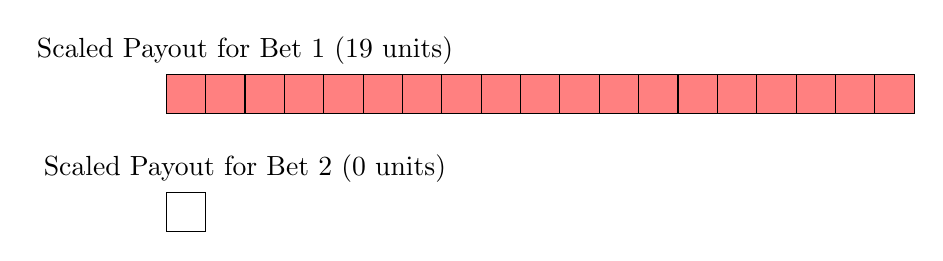
\begin{tikzpicture}[scale=0.5]

% Scaled Payout for Bet 1 (NO)
\foreach \x in {1,...,19}
{
    \draw[fill=red!50] (\x,0) rectangle ++(1,1);
}

% Label for Scaled Payout of Bet 1
\node[above] at (3,1) {Scaled Payout for Bet 1 (\( 19 \text{ units} \))};

% Scaled Payout for Bet 2 (YES)
\foreach \x in {1,...,1}
{
    \draw[fill=white!50] (\x,-3) rectangle ++(1,1);
}

% Label for Scaled Payout of Bet 2
\node[above] at (3,-2) {Scaled Payout for Bet 2 (\( 0 \text{ units} \))};

\end{tikzpicture}
\end{center}

\section*{Adjust Payouts Equations}

\subsection*{Calculate Excess}

The excess is the difference between the total scaled payouts and the available pool of funds in the market:

\[
\text{Excess} = \sum_{i=1}^{n} \text{ScaledPayout}_i - \text{AvailablePool}
\]

Where:
\begin{itemize}
    \item \( \text{ScaledPayout}_i \): The scaled payout for the \(i\)-th bet.
    \item \( \text{AvailablePool} \): The total available pool of funds, calculated as:
    \[
    \text{AvailablePool} = \text{MarketVolume}(\text{Bets})
    \]
\end{itemize}


\subsection*{Calculate Excess}

\textbf{Given:}

\begin{itemize}
    \item Scaled Payouts:
    \begin{itemize}
        \item \( \text{Scaled Payout}_{\text{NO,1}} = 19 \text{ units} \)
        \item \( \text{Scaled Payout}_{\text{YES,2}} = 0 \text{ units} \)
    \end{itemize}
    \item Available Pool:
    \[
    \text{Available Pool} = \text{Sum of Bets} = 20 + 10 = 30 \text{ units}
    \]
\end{itemize}

\textbf{Excess Calculation:}

\[
\text{Excess} = \sum_{i=1}^{n} \text{Scaled Payout}_i - \text{Available Pool}
\]

\[
\text{Excess} = (19 + 0) - 30
\]

\[
\text{Excess} = 19 - 30 = -11 \text{ units}
\]

\textbf{Interpretation:}

Since the calculated \textbf{Excess} is negative (\( \text{Excess} < 0 \)), this indicates that the scaled payouts are \( 11 \text{ units} \) below the available pool, requiring adjustments to redistribute this shortfall across the payouts to align with the total pool.

\subsection*{Adjust for Positive Excess}

If the calculated excess is positive (\(\text{Excess} > 0\)), we adjust the payouts by deducting from the newest payouts (starting from the last):

\[
\text{If Excess} > 0:
\]

\[
\text{For } i = n, n-1, \dots, 1, \text{ while Excess} > 0:
\]
\[
\text{If ScaledPayout}_i > 0, \text{ then:}
\]
\[
\text{ScaledPayout}_i \gets \text{ScaledPayout}_i - 1
\]
\[
\text{Excess} \gets \text{Excess} - 1
\]

The adjustment continues until \(\text{Excess} = 0\).

In our scenario above, we have no positive excess so we don't need to calculate it.

\subsection*{Adjust for Negative Excess}

If the calculated excess is negative (\(\text{Excess} < 0\)), we adjust the payouts by adding to the oldest payouts (starting from the first):

\[
\text{If Excess} < 0:
\]

\[
\text{For } i = 1, 2, \dots, n, \text{ while Excess} < 0:
\]
\[
\text{ScaledPayout}_i \gets \text{ScaledPayout}_i + 1
\]
\[
\text{Excess} \gets \text{Excess} + 1
\]

The adjustment continues until \(\text{Excess} = 0\).

\subsection*{Adjust for Negative Excess}

If the calculated excess is negative (\(\text{Excess} < 0\)), we adjust the payouts by incrementing all payouts cyclically, starting from the oldest, until the excess is resolved:

\[
\text{If Excess} < 0:
\]

\[
\text{While Excess} < 0:
\]
\[
\text{For } i = 1, 2, \dots, n:
\]
\[
\text{ScaledPayout}_i \gets \text{ScaledPayout}_i + 1
\]
\[
\text{Excess} \gets \text{Excess} + 1
\]

\textbf{Given:}

\begin{itemize}
    \item Initial Scaled Payouts:
    \[
    \text{Scaled Payout}_{\text{NO,1}} = 19, \quad \text{Scaled Payout}_{\text{YES,2}} = 0
    \]
    \item Initial Excess:
    \[
    \text{Excess} = -11
    \]
\end{itemize}

\textbf{Step-by-Step Adjustment:}

We cycle through the payouts, adding \(+1\) to each in turn, until the excess is resolved:

\begin{itemize}
    \item Cycle 1:
    \begin{align*}
        \text{Scaled Payout}_{\text{NO,1}} &= 19 + 1 = 20 \\
        \text{Scaled Payout}_{\text{YES,2}} &= 0 + 1 = 1 \\
        \text{Excess} &= -11 + 2 = -9
    \end{align*}
    \item Cycle 2:
    \begin{align*}
        \text{Scaled Payout}_{\text{NO,1}} &= 20 + 1 = 21 \\
        \text{Scaled Payout}_{\text{YES,2}} &= 1 + 1 = 2 \\
        \text{Excess} &= -9 + 2 = -7
    \end{align*}
    \item Cycle 3:
    \begin{align*}
        \text{Scaled Payout}_{\text{NO,1}} &= 21 + 1 = 22 \\
        \text{Scaled Payout}_{\text{YES,2}} &= 2 + 1 = 3 \\
        \text{Excess} &= -7 + 2 = -5
    \end{align*}
    \item Cycle 4:
    \begin{align*}
        \text{Scaled Payout}_{\text{NO,1}} &= 22 + 1 = 23 \\
        \text{Scaled Payout}_{\text{YES,2}} &= 3 + 1 = 4 \\
        \text{Excess} &= -5 + 2 = -3
    \end{align*}
    \item Cycle 5:
    \begin{align*}
        \text{Scaled Payout}_{\text{NO,1}} &= 23 + 1 = 24 \\
        \text{Scaled Payout}_{\text{YES,2}} &= 4 + 1 = 5 \\
        \text{Excess} &= -3 + 2 = -1
    \end{align*}
    \item Final Cycle:
    \begin{align*}
        \text{Scaled Payout}_{\text{NO,1}} &= 24 + 1 = 25 \\
        \text{Scaled Payout}_{\text{YES,2}} &= 5 \quad (\text{unchanged}) \\
        \text{Excess} &= -1 + 1 = 0
    \end{align*}
\end{itemize}

\textbf{Final Adjusted Scaled Payouts:}

\[
\text{Scaled Payout}_{\text{NO,1}} = 25, \quad \text{Scaled Payout}_{\text{YES,2}} = 5
\]

\textbf{Adjusted Excess:}

\[
\text{Excess} = (25 + 5) - 30 = 30 - 30 = 0
\]

\textbf{Interpretation:}

The excess of \(-11\) has been evenly redistributed across the payouts by cyclically adding \(+1\) to each, starting with the oldest (\(\text{NO,1}\)), until the excess reached \(0\).

\textbf{Final Adjusted Scaled Payouts:}

\[
\text{Scaled Payout}_{\text{NO,1}} = 25, \quad \text{Scaled Payout}_{\text{YES,2}} = 5
\]

\textbf{Adjusted Excess:}

\[
\text{Excess} = (25 + 5) - 30 = 30 - 30 = 0
\]

\textbf{Interpretation:}

The negative excess has been resolved by distributing the excess equally between the payouts for \(\text{NO}\) and \(\text{YES}\), ensuring the total scaled payouts match the available pool.


\subsection*{Adjust Payouts Function}

The overall adjustment process is summarized as follows:

\[
\text{Excess} \gets \sum_{i=1}^{n} \text{ScaledPayout}_i - \text{AvailablePool}
\]

\[
\text{If Excess} > 0:
\]
\[
\text{Adjust payouts using AdjustForPositiveExcess.}
\]

\[
\text{Else if Excess} < 0:
\]
\[
\text{Adjust payouts using AdjustForNegativeExcess.}
\]

\[
\text{Return Adjusted ScaledPayouts.}
\]



% Double Divider Line To Next Step
\begin{center}
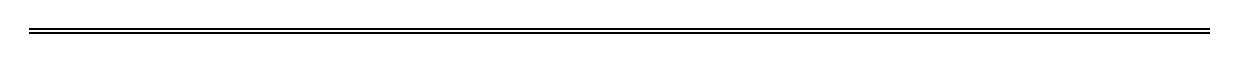
\begin{tikzpicture}[scale=0.5]
\draw[thick] (0,-1) -- (30,-1);
\draw[thick] (0,-1.1) -- (30,-1.1);
\end{tikzpicture}
\end{center}

\newpage

\section{Third Transaction}

\begin{itemize}
    \item \textbf{Third Transaction:} Another bettor places 10 units in the YES direction.
\end{itemize}

\begin{center}
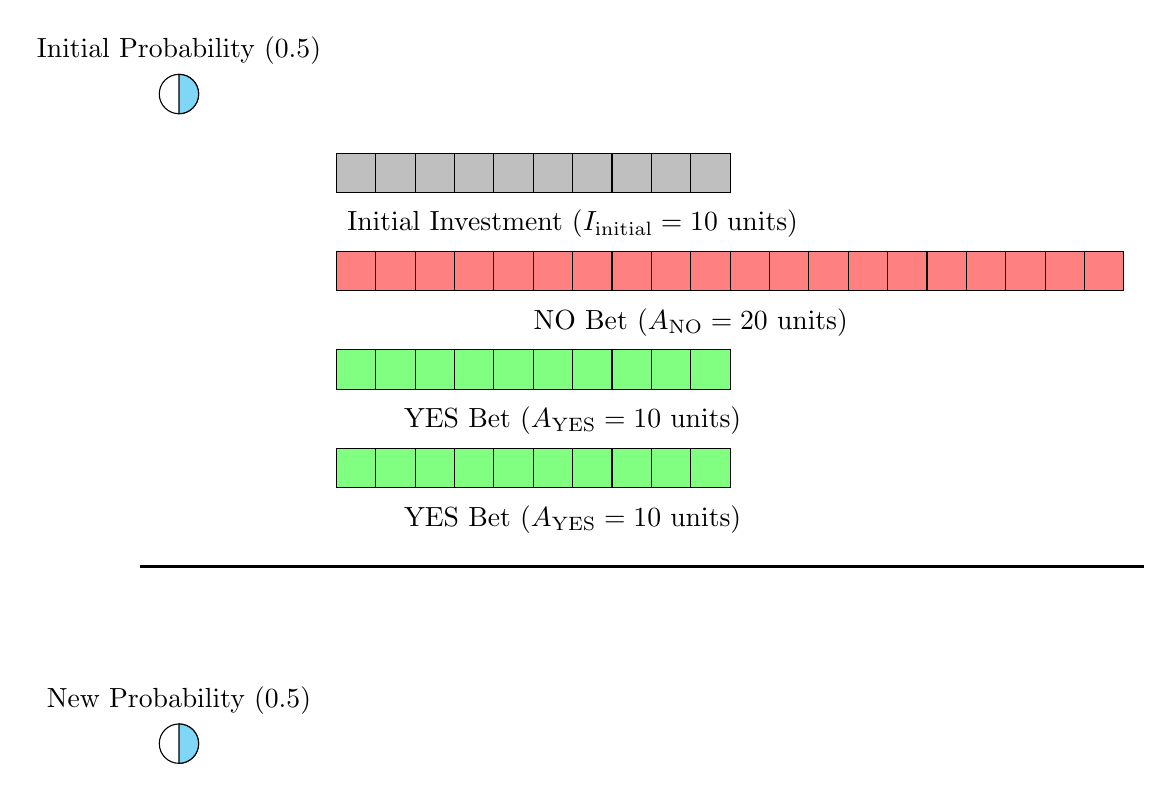
\begin{tikzpicture}[scale=0.5]

% Pie Chart for Initial Probability 0.5 at x = -1, y = 2.5
\piechart{-1}{2.5}{0.5}
\node[above] at (-1,3) {Initial Probability (0.5)};

% Pie Chart for New Probability 0.5 at x = -1, y = -14
\piechart{-1}{-14}{0.5}
\node[above] at (-1,-13.5) {New Probability (0.5)};

% Initial Investment (Gray Squares)
\foreach \x in {3,...,12}
{
    \draw[fill=gray!50] (\x,0) rectangle ++(1,1);
}

% YES Bet (Green Squares), first YES bet, set down by -5
\foreach \x in {3,...,12}
{
    \draw[fill=green!50] (\x,-5) rectangle ++(1,1);
}

% YES Bet (Green Squares), second YES bet, set down by -7.5
\foreach \x in {3,...,12}
{
    \draw[fill=green!50] (\x,-7.5) rectangle ++(1,1);
}

% NO Bet (Red Squares), set down by -2.5
\foreach \x in {3,...,22}
{
    \draw[fill=red!50] (\x,-2.5) rectangle ++(1,1);
}

% Horizontal Line between the squares
\draw[thick] (-2,-9.5) -- (23.5,-9.5);

% Labels
\node[below] at (9,-0.2) {Initial Investment (\(I_{\text{initial}} = 10\) units)};
\node[below] at (12,-2.7) {NO Bet (\(A_{\text{NO}} = 20\) units)};
\node[below] at (9,-5.2) {YES Bet (\(A_{\text{YES}} = 10\) units)};
\node[below] at (9,-7.7) {YES Bet (\(A_{\text{YES}} = 10\) units)};

\end{tikzpicture}
\end{center}

\[
P_{\text{new}} = \frac{0.5 \times 10 + 20}{10 + 20 + 20} = \frac{25}{50} = 0.5
\]

\subsection*{Market Share Division}

\[
S = \text{Total Market Volume} + I_{\text{initial}} = (20 + 20) = 40 \text{ units}
\]

\begin{align*}
S_{\text{YES}} &= \left\lfloor S \times P_{\text{new}} \right\rceil = \left\lfloor 50 \times 0.5 \right\rceil = 20 \\
S_{\text{NO}} &= \left\lfloor S \times (1 - P_{\text{new}}) \right\rceil = \left\lfloor 50 \times 0.5 \right\rceil = 20
\end{align*}

\begin{center}
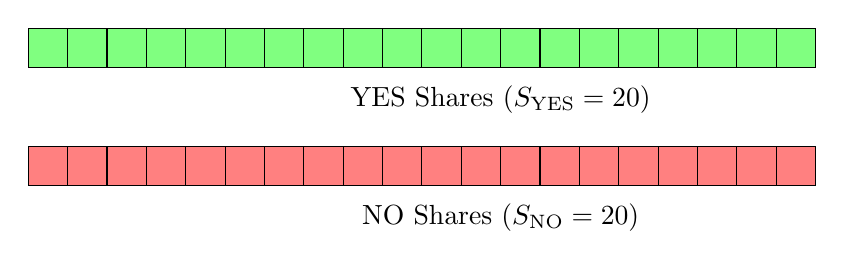
\begin{tikzpicture}[scale=0.5]

% YES Shares (Green Squares), set down by -12
\foreach \x in {1,...,20}
{
    \draw[fill=green!50] (\x,-12) rectangle ++(1,1);
}

% NO Shares (Red Squares), set down by -15
\foreach \x in {1,...,20}
{
    \draw[fill=red!50] (\x,-15) rectangle ++(1,1);
}

% Labels
\node[below] at (13,-12.2) {YES Shares (\(S_{\text{YES}} = 20\))};
\node[below] at (13,-15.2) {NO Shares (\(S_{\text{NO}} = 20\))};

\end{tikzpicture}

\end{center}


\section*{Calculating Course Payouts}

\subsection*{Step One: Calculate Reward Factor for Each Bet}

\[
d_i = |R - p_i|
\]

\subsection*{Step Two: Calculate Course Payout for Each Bet}

\[
C_i = d_i \times b_i
\]

\subsection*{Example Calculations for Third Transaction}

\textbf{Given:}

\begin{itemize}
  \item Resolution Probability: \( R = 0.5 \)
  \item Bet 0: Neutral, \( b_0 = 10 \) units, \( p_0 = 0.5 \)
  \item Bet 1: NO, \( b_1 = 20 \) units, \( p_1 = 0.167 \)
  \item Bet 2: YES, \( b_2 = 10 \) units, \( p_2 = 0.375 \)
  \item Bet 3: YES, \( b_3 = 10 \) units, \( p_3 = 0.5 \)
\end{itemize}

\textbf{For Bet 1:}

\[
d_1 = |R - p_1| = |0.5 - 0.167| = 0.333
\]
\[
C_1 = d_1 \times b_1 = 0.333 \times 20 = 6.660 \text{ units}
\]

\textbf{For Bet 2:}

\[
d_2 = |R - p_2| = |0.5 - 0.375| = 0.125
\]
\[
C_2 = d_2 \times b_2 = 0.125 \times 10 = 1.250 \text{ units}
\]

\textbf{For Bet 3:}

\[
d_3 = |R - p_3| = |0.5 - 0.5| = 0
\]
\[
C_3 = d_3 \times b_3 = 0 \times 10 = 0 \text{ units}
\]

\begin{center}
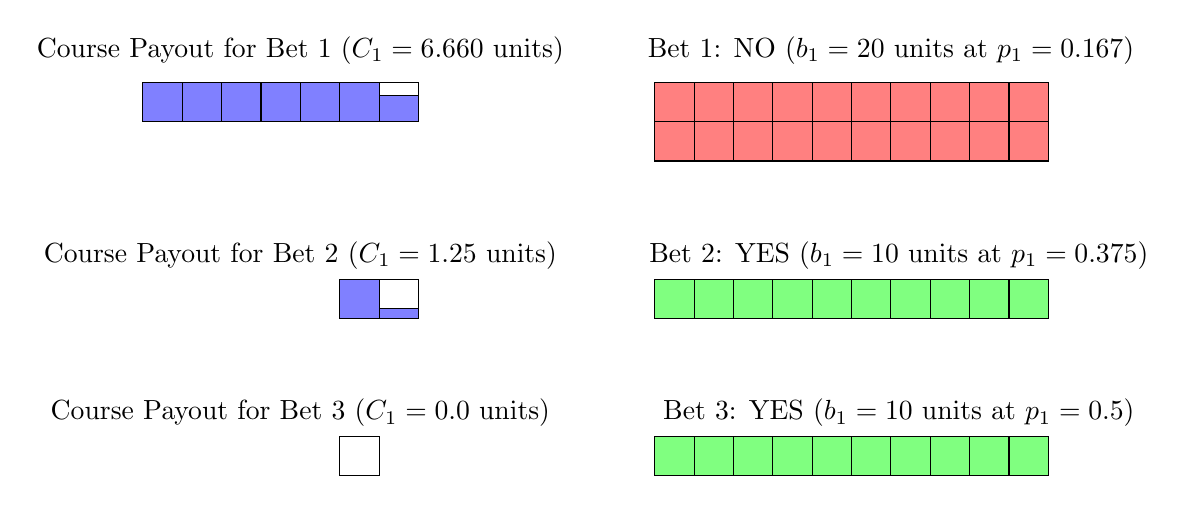
\begin{tikzpicture}[scale=0.5]

% Bet 1: NO Bet (Red Squares), starting at x = 5
\foreach \x in {5,...,14}
{
    \draw[fill=red!50] (\x,0) rectangle ++(1,1);
    \draw[fill=red!50] (\x,-1) rectangle ++(1,1);
}

% Label for Bet 1
\node[above] at (11,1.2) {Bet 1: NO (\( b_1 = 20 \) units at \( p_1 = 0.167 \))};

% Course Payout for Bet 1 (Blue Squares)
\foreach \x in {-8,...,-3}
{
    \draw (\x,0) rectangle ++(1,1);
    \filldraw[fill=blue!50] (\x,0) rectangle ++(1,1);
}

% Course Payout for Bet 1 (Blue Squares)
\def\xPartial{-2}
\draw (\xPartial,0) rectangle ++(1,1);
\filldraw[fill=blue!50] (\xPartial,0) rectangle ++(1,0.66);

% Label for Course Payout of Bet 1
\node[above] at (-4,1.2) {Course Payout for Bet 1 (\( C_1 = 6.660 \) units)};

% Bet 2 YES (Green Squares)
\foreach \x in {5,...,14}
{
    \draw[fill=green!50] (\x,-5) rectangle ++(1,1);
}

% Label for Bet 2
\node[above] at (11.2,-4) {Bet 2: YES (\( b_1 = 10 \) units at \( p_1 = 0.375 \))};


% Course Payout for Bet 2 (Blue Squares)
\foreach \x in {-3,...,-3}
{
    \draw (\x,-5) rectangle ++(1,1);
    \filldraw[fill=blue!50] (\x,-5) rectangle ++(1,1);
}

% Partial Course Payout for Bet 2 (Blue Squares)
\def\xPartial{-2}
\draw (\xPartial,-5) rectangle ++(1,1);
\filldraw[fill=blue!50] (\xPartial,-5) rectangle ++(1,0.25);

% Label for Course Payout of Bet 2
\node[above] at (-4,-4) {Course Payout for Bet 2 (\( C_1 = 1.25 \) units)};


% Bet 3 YES (Green Squares)
\foreach \x in {5,...,14}
{
    \draw[fill=green!50] (\x,-9) rectangle ++(1,1);
}

% Label for Bet 3
\node[above] at (11.2,-8) {Bet 3: YES (\( b_1 = 10 \) units at \( p_1 = 0.5 \))};

% Course Payout for Bet 3
\def\xPartial{-3}  % Position of the partial square
\draw (\xPartial,-9) rectangle ++(1,1);

% Label for Course Payout of Bet 3
\node[above] at (-4,-8) {Course Payout for Bet 3 (\( C_1 = 0.0 \) units)};


\end{tikzpicture}
\end{center}


\newpage

\section*{Normalization Factor Calculation for Third Transaction}

\subsection*{Step Three: Calculate Normalization Factor}

Given:
\begin{itemize}
    \item Total YES Shares: \( S_{\text{YES}} = 25 \)
    \item Total NO Shares: \( S_{\text{NO}} = 25 \)
    \item Course Payouts:
    \begin{itemize}
        \item \( C_{\text{NO,1}} = 6.66 \) units
        \item \( C_{\text{YES,1}} = 1.25 \) units
        \item \( C_{\text{YES,2}} = 0 \) units
        \item Total payout sums: \( C_{\text{YES\_SUM}} = 1.25 \), \( C_{\text{NO\_SUM}} = 6.66 \)
    \end{itemize}
\end{itemize}

\subsubsection*{Calculate YES Normalization Factor}

\[
F_{\text{YES}} =
\begin{cases}
      \frac{S_{\text{YES}}}{C_{\text{YES\_SUM}}} & \text{if } C_{\text{YES\_SUM}} > 0 \\
      0 & \text{if } C_{\text{YES\_SUM}} = 0
   \end{cases}
\]

Since \( C_{\text{YES\_SUM}} = 1.25 \), we have:

\[
F_{\text{YES}} = \frac{20}{1.25} = 16
\]

\subsubsection*{Calculate NO Normalization Factor}

\[
F_{\text{NO}} =
\begin{cases}
      \frac{S_{\text{NO}}}{C_{\text{NO\_SUM}}} & \text{if } C_{\text{NO\_SUM}} > 0 \\
      0 & \text{if } C_{\text{NO\_SUM}} = 0
   \end{cases}
\]

Since \( C_{\text{NO\_SUM}} = 6.66 \), we have:

\[
F_{\text{NO}} = \frac{20}{6.66} \approx 3.00
\]

Thus, the normalization factors are:

\[
F_{\text{YES}} = 16, \quad F_{\text{NO}} \approx 3.00
\]

% Double Divider Line To Next Step
\begin{center}
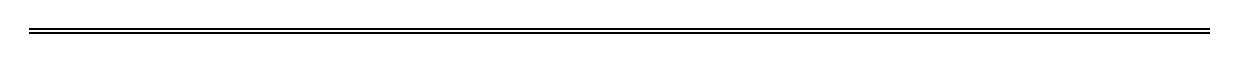
\begin{tikzpicture}[scale=0.5]
\draw[thick] (0,-1) -- (30,-1);
\draw[thick] (0,-1.1) -- (30,-1.1);
\end{tikzpicture}
\end{center}

\newpage


\section*{Scaled Payout Calculation for Third Transaction}

\begin{itemize}
    \item \textbf{Purpose of Scaled Payouts:}
    \begin{itemize}
        \item Scaled payouts adjust raw course payouts proportionally based on normalization factors to ensure payouts align with the available shares in the market pool.
        \item The adjustment ensures fairness, reflecting the market's allocation of shares while staying within constraints.
        \item Scaled payouts provide accurate distributions of rewards based on contributions and probabilities in the market.
    \end{itemize}
\end{itemize}

\subsection*{Step Four: Calculate Scaled Payout for Each Bet}

Given:
\begin{itemize}
    \item Normalization Factors: \( F_{\text{YES}} = 20 \), \( F_{\text{NO}} \approx 3.75 \)
    \item Course Payouts:
    \begin{itemize}
        \item \( C_{\text{NO,1}} = 6.66 \) units
        \item \( C_{\text{YES,2}} = 1.25 \) units
        \item \( C_{\text{YES,3}} = 0 \) units
    \end{itemize}
\end{itemize}

\textbf{For Bet 1 (NO):}

\[
\text{Scaled Payout}_{\text{NO,1}} = \text{Round}(C_{\text{NO,1}} \times F_{\text{NO}})
\]
\[
\text{Scaled Payout}_{\text{NO,1}} = \text{Round}(6.66 \times 3.00) = \text{Round}(20.000) = 20 \text{ units}
\]

\textbf{For Bet 2 (YES):}

\[
\text{Scaled Payout}_{\text{YES,2}} = \text{Round}(C_{\text{YES,2}} \times F_{\text{YES}})
\]
\[
\text{Scaled Payout}_{\text{YES,2}} = \text{Round}(1.25 \times 16) = \text{Round}(20.00) = 20 \text{ units}
\]

\textbf{For Bet 3 (YES):}

\[
\text{Scaled Payout}_{\text{YES,3}} = \text{Round}(C_{\text{YES,3}} \times F_{\text{YES}})
\]
\[
\text{Scaled Payout}_{\text{YES,3}} = \text{Round}(0 \times 20) = \text{Round}(0) = 0 \text{ units}
\]

\subsubsection*{Final Scaled Payouts:}
\[
\text{Bet 1 (NO): } 20 \text{ units}
\]
\[
\text{Bet 2 (YES): } 20 \text{ units}
\]
\[
\text{Bet 3 (YES): } 0 \text{ units}
\]

\begin{center}
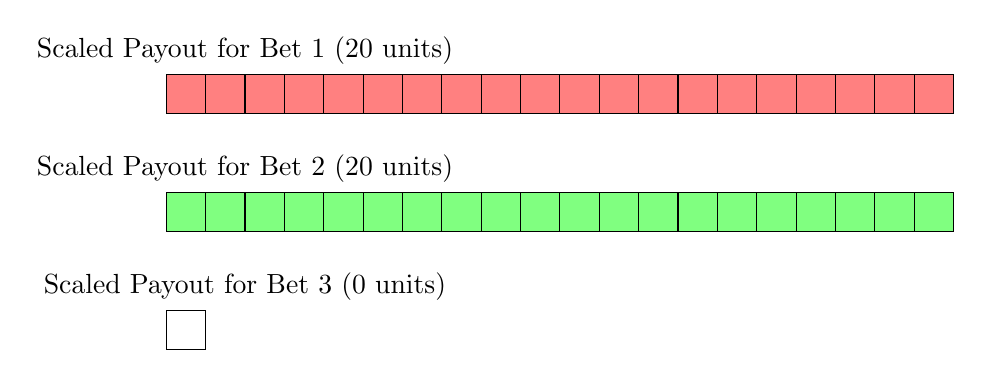
\begin{tikzpicture}[scale=0.5]

% Scaled Payout for Bet 1 (NO)
\foreach \x in {1,...,20}
{
    \draw[fill=red!50] (\x,0) rectangle ++(1,1);
}

% Label for Scaled Payout of Bet 1
\node[above] at (3,1) {Scaled Payout for Bet 1 (\( 20 \text{ units} \))};

% Scaled Payout for Bet 2 (YES)
\foreach \x in {1,...,20}
{
    \draw[fill=green!50] (\x,-3) rectangle ++(1,1);
}

% Label for Scaled Payout of Bet 2
\node[above] at (3,-2) {Scaled Payout for Bet 2 (\( 20 \text{ units} \))};

% Scaled Payout for Bet 3 (YES)
\foreach \x in {1,...,1}
{
    \draw[fill=white!50] (\x,-6) rectangle ++(1,1);
}

% Label for Scaled Payout of Bet 3
\node[above] at (3,-5) {Scaled Payout for Bet 3 (\( 0 \text{ units} \))};

\end{tikzpicture}
\end{center}



\newpage

% --------------------- Fourth Transaction ---------------------

\section{Fourth Transaction}

\begin{itemize}
    \item \textbf{Fourth Transaction:} The original bettor holding NO sells 10 units of NO.
\end{itemize}

\begin{center}
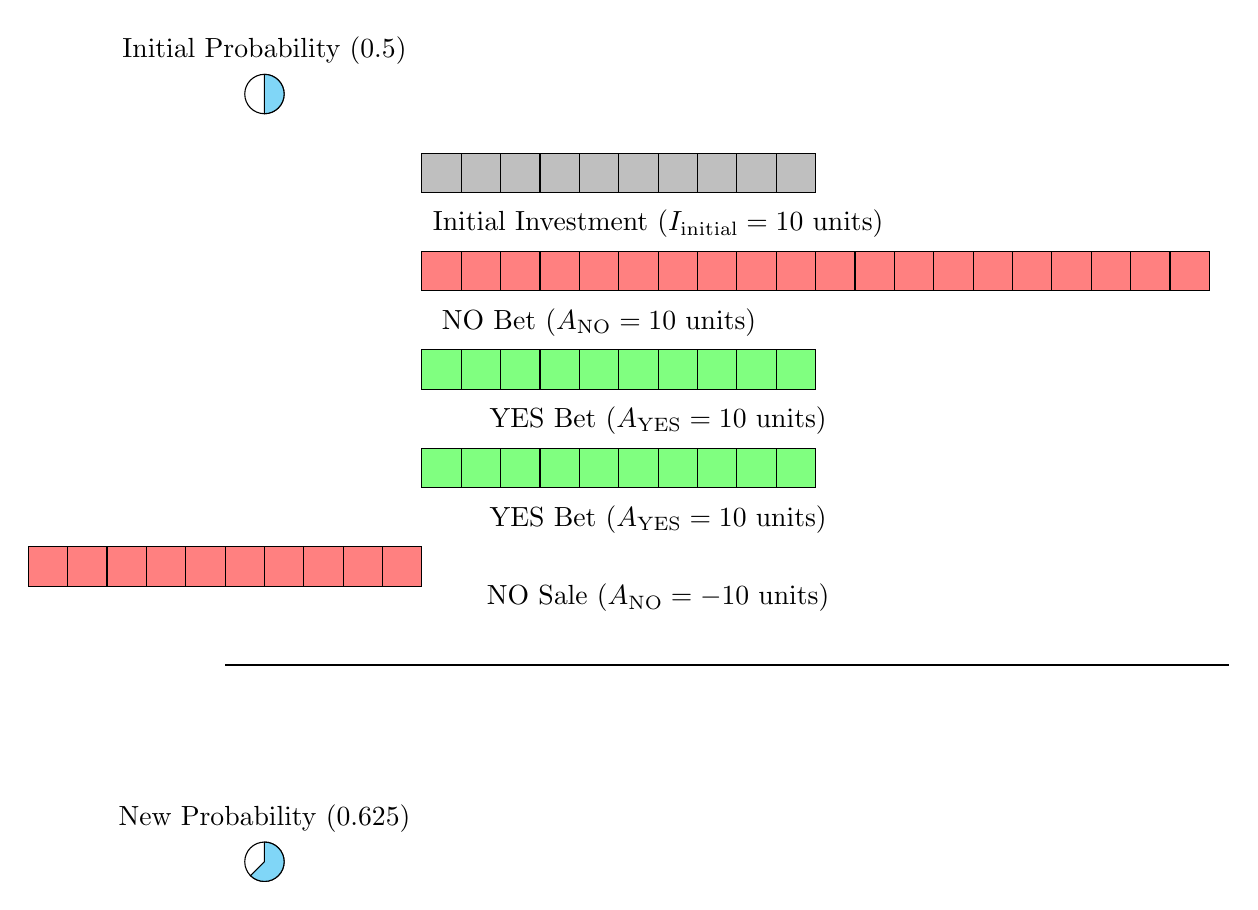
\begin{tikzpicture}[scale=0.5]

% Pie Chart for Initial Probability 0.5 at x = -1, y = 2.5
\piechart{-1}{2.5}{0.5}
\node[above] at (-1,3) {Initial Probability (0.5)};

% Pie Chart for New Probability 0.625 at x = -1, y = -17
\piechart{-1}{-17}{0.625}
\node[above] at (-1,-16.5) {New Probability (0.625)};

% Initial Investment (Gray Squares)
\foreach \x in {3,...,12}
{
    \draw[fill=gray!50] (\x,0) rectangle ++(1,1);
}

% NO Bet (Red Squares), set down by -2.5
\foreach \x in {3,...,22}
{
    \draw[fill=red!50] (\x,-2.5) rectangle ++(1,1);
}


% YES Bet (Green Squares), first YES bet, set down by -5
\foreach \x in {3,...,12}
{
    \draw[fill=green!50] (\x,-5) rectangle ++(1,1);
}

% YES Bet (Green Squares), second YES bet, set down by -7.5
\foreach \x in {3,...,12}
{
    \draw[fill=green!50] (\x,-7.5) rectangle ++(1,1);
}


% Negative NO Bet (Red Squares)
\foreach \x in {2,...,-7}
{
    \draw[fill=red!50] (\x,-10) rectangle ++(1,1);
}


% Horizontal Line between the squares
\draw[thick] (-2,-12.0) -- (23.5,-12.0);


% Labels
\node[below] at (9,-0.2) {Initial Investment (\(I_{\text{initial}} = 10\) units)};
\node[below] at (7.5,-2.7) {NO Bet (\(A_{\text{NO}} = 10\) units)};
\node[below] at (9,-5.2) {YES Bet (\(A_{\text{YES}} = 10\) units)};
\node[below] at (9,-7.7) {YES Bet (\(A_{\text{YES}} = 10\) units)};
\node[below] at (9,-9.7) {NO Sale (\(A_{\text{NO}} = -10\) units)};

\end{tikzpicture}
\end{center}

\[
P_{\text{new}} = \frac{0.5 \times 10 + 20}{10 + 20} = \frac{25}{40} = 0.625
\]

\subsection*{Market Share Division}

\[
S = \text{Total Market Volume} + I_{\text{initial}} = (20 + 10) = 30 \text{ units}
\]

\begin{align*}
S_{\text{YES}} &= \left\lfloor S \times P_{\text{new}} \right\rceil = \left\lfloor 30 \times 0.625 \right\rceil = 19 \\
S_{\text{NO}} &= \left\lfloor S \times (1 - P_{\text{new}}) \right\rceil = \left\lfloor 30 \times 0.375 \right\rceil = 11
\end{align*}

\begin{center}
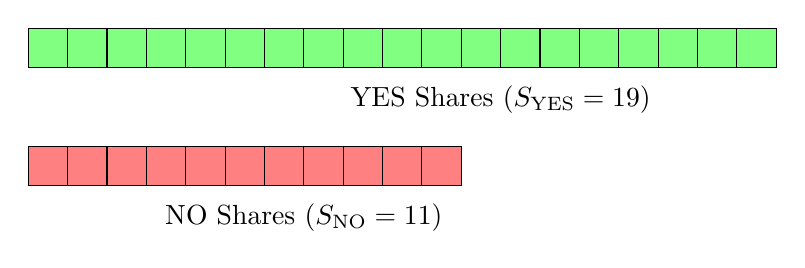
\begin{tikzpicture}[scale=0.5]

% YES Shares (Green Squares), set down by -17
\foreach \x in {1,...,19}
{
    \draw[fill=green!50] (\x,-17) rectangle ++(1,1);
}

% NO Shares (Red Squares), set down by -20
\foreach \x in {1,...,11}
{
    \draw[fill=red!50] (\x,-20) rectangle ++(1,1);
}

% Labels
\node[below] at (13,-17.2) {YES Shares (\(S_{\text{YES}} = 19\))};
\node[below] at (8,-20.2) {NO Shares (\(S_{\text{NO}} = 11\))};

\end{tikzpicture}
\end{center}

\section*{Calculating Course Payouts}


\subsection*{Step One: Calculate Reward Factor for Each Bet}

\[
d_i = |R - p_i|
\]

\subsection*{Step Two: Calculate Course Payout for Each Bet}

\[
C_i = d_i \times b_i
\]

\subsection*{Example Calculations for Fourth Transaction}

\textbf{Given:}

\begin{itemize}
  \item Resolution Probability: \( R = 0.625 \)
  \item Bet 0: Neutral, \( b_0 = 10 \) units, \( p_0 = 0.5 \)
  \item Bet 1: NO, \( b_1 = 20 \) units, \( p_1 = 0.167 \)
  \item Bet 2: YES, \( b_2 = 10 \) units, \( p_2 = 0.375 \)
  \item Bet 3: YES, \( b_3 = 10 \) units, \( p_3 = 0.5 \)
  \item Bet 4: NO Sale, \( b_4 = -10 \) units, \( p_4 = 0.625 \)
\end{itemize}

\textbf{For Bet 1:}

\[
d_1 = |R - p_1| = |0.625 - 0.167| = 0.458
\]
\[
C_1 = d_1 \times b_1 = 0.458 \times 20 = 9.16 \text{ units}
\]

\textbf{For Bet 2:}

\[
d_2 = |R - p_2| = |0.625 - 0.375| = 0.25
\]
\[
C_2 = d_2 \times b_2 = 0.25 \times 10 = 2.5 \text{ units}
\]

\textbf{For Bet 3:}

\[
d_3 = |R - p_3| = |0.625 - 0.5| = 0.125
\]
\[
C_3 = d_3 \times b_3 = 0.125 \times 10 = 1.25 \text{ units}
\]

\textbf{For Bet 4:}

\[
d_4 = |R - p_4| = |0.625 - 0.625| = 0
\]
\[
C_4 = d_4 \times b_4 = 0 \times (-10) = 0 \text{ units}
\]


\begin{center}
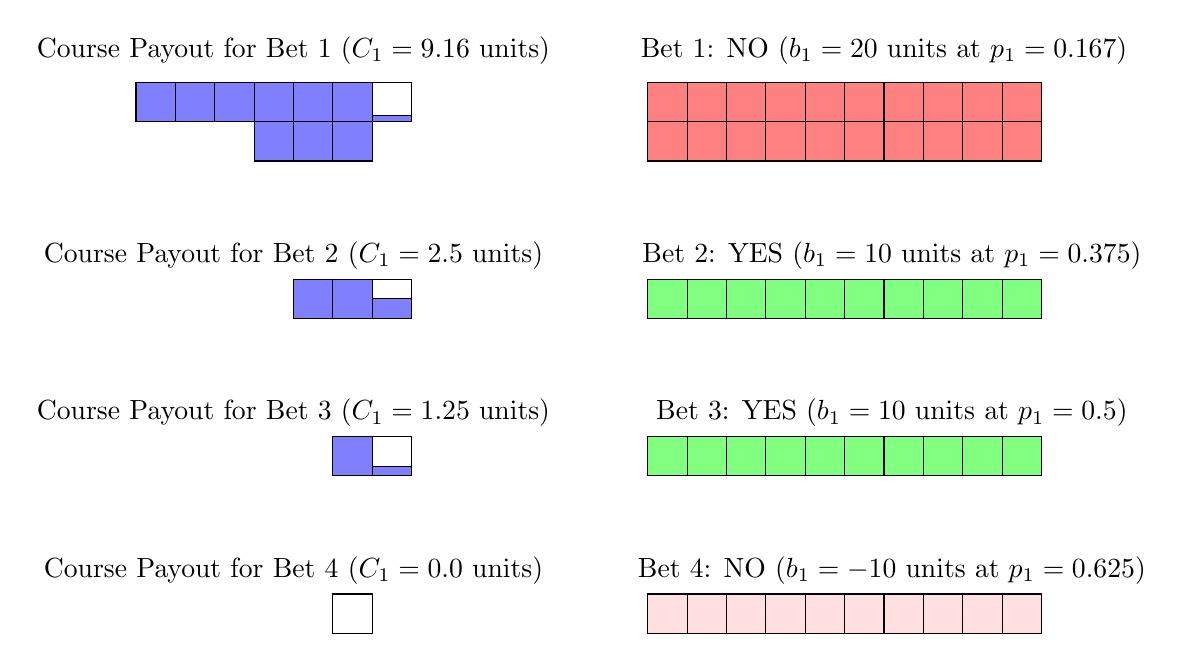
\begin{tikzpicture}[scale=0.5]

% Bet 1: NO Bet (Red Squares), starting at x = 5
\foreach \x in {5,...,14}
{
    \draw[fill=red!50] (\x,0) rectangle ++(1,1);
    \draw[fill=red!50] (\x,-1) rectangle ++(1,1);
}

% Label for Bet 1
\node[above] at (11,1.2) {Bet 1: NO (\( b_1 = 20 \) units at \( p_1 = 0.167 \))};

% Course Payout for Bet 1 (Blue Squares)
\foreach \x in {-8,...,-3}
{
    \draw (\x,0) rectangle ++(1,1);
    \filldraw[fill=blue!50] (\x,0) rectangle ++(1,1);
}
\foreach \x in {-5,...,-3}
{
    \draw (\x,0) rectangle ++(1,1);
    \filldraw[fill=blue!50] (\x,-1) rectangle ++(1,1);
}

% Course Payout for Bet 1 (Blue Squares)
\def\xPartial{-2}
\draw (\xPartial,0) rectangle ++(1,1);
\filldraw[fill=blue!50] (\xPartial,0) rectangle ++(1,0.16);

% Label for Course Payout of Bet 1
\node[above] at (-4,1.2) {Course Payout for Bet 1 (\( C_1 = 9.16 \) units)};

% Bet 2 YES (Green Squares)
\foreach \x in {5,...,14}
{
    \draw[fill=green!50] (\x,-5) rectangle ++(1,1);
}

% Label for Bet 2
\node[above] at (11.2,-4) {Bet 2: YES (\( b_1 = 10 \) units at \( p_1 = 0.375 \))};


% Course Payout for Bet 2 (Blue Squares)
\foreach \x in {-4,...,-3}
{
    \draw (\x,-5) rectangle ++(1,1);
    \filldraw[fill=blue!50] (\x,-5) rectangle ++(1,1);
}

% Partial Course Payout for Bet 2 (Blue Squares)
\def\xPartial{-2}
\draw (\xPartial,-5) rectangle ++(1,1);
\filldraw[fill=blue!50] (\xPartial,-5) rectangle ++(1,0.5);

% Label for Course Payout of Bet 2
\node[above] at (-4,-4) {Course Payout for Bet 2 (\( C_1 = 2.5 \) units)};


% Bet 3 YES (Green Squares)
\foreach \x in {5,...,14}
{
    \draw[fill=green!50] (\x,-9) rectangle ++(1,1);
}

% Partial Course Payout for Bet 3 (Blue Squares)
\def\xPartial{-2}
\draw (\xPartial,-9) rectangle ++(1,1);
\filldraw[fill=blue!50] (\xPartial,-9) rectangle ++(1,0.25);


% Label for Bet 3
\node[above] at (11.2,-8) {Bet 3: YES (\( b_1 = 10 \) units at \( p_1 = 0.5 \))};


% Course Payout for Bet 3
\foreach \x in {-3,...,-3}
{
    \draw (\x,-9) rectangle ++(1,1);
    \filldraw[fill=blue!50] (\x,-9) rectangle ++(1,1);
}



% Label for Course Payout of Bet 3
\node[above] at (-4,-8) {Course Payout for Bet 3 (\( C_1 = 1.25 \) units)};


% Bet 4 YES (Red Squares)
\foreach \x in {5,...,14}
{
    \draw[fill=pink!50] (\x,-13) rectangle ++(1,1);
}

% Label for Bet 4
\node[above] at (11.2,-12) {Bet 4: NO (\( b_1 = -10 \) units at \( p_1 = 0.625 \))};

% Course Payout for Bet 4
\def\xPartial{-3}  % Position of the partial square
\draw (\xPartial,-13) rectangle ++(1,1);

% Label for Course Payout of Bet 4
\node[above] at (-4,-12) {Course Payout for Bet 4 (\( C_1 = 0.0 \) units)};



\end{tikzpicture}
\end{center}

\section*{Normalization Factor Calculation for Fourth Transaction}

\subsection*{Step Three: Calculate Normalization Factor}

Given:
\begin{itemize}
    \item Total YES Shares: \( S_{\text{YES}} = 19 \)
    \item Total NO Shares: \( S_{\text{NO}} = 11 \)
    \item Course Payouts:
    \begin{itemize}
        \item \( C_{\text{YES,1}} = 2.5 \) units
        \item \( C_{\text{NO,1}} = 9.16 \) units
        \item \( C_{\text{YES,2}} = 1.25 \) units
        \item \( C_{\text{NO,2}} = 0.0 \) units
        \item Total payout sums: \( C_{\text{YES\_SUM}} = 3.75 \), \( C_{\text{NO\_SUM}} = 9.16 \)
    \end{itemize}
\end{itemize}

\subsubsection*{Calculate YES Normalization Factor}

\[
F_{\text{YES}} =
\begin{cases}
      \frac{S_{\text{YES}}}{C_{\text{YES\_SUM}}} & \text{if } C_{\text{YES\_SUM}} > 0 \\
      0 & \text{if } C_{\text{YES\_SUM}} = 0
   \end{cases}
\]

Since \( C_{\text{YES\_SUM}} = 3.75 \), we have:

\[
F_{\text{YES}} = \frac{19}{3.75} = 5.067
\]

\subsubsection*{Calculate NO Normalization Factor}

\[
F_{\text{NO}} =
\begin{cases}
      \frac{S_{\text{NO}}}{C_{\text{NO\_SUM}}} & \text{if } C_{\text{NO\_SUM}} > 0 \\
      0 & \text{if } C_{\text{NO\_SUM}} = 0
   \end{cases}
\]

Since \( C_{\text{NO\_SUM}} = 9.16 \), we have:

\[
F_{\text{NO}} = \frac{11}{9.16} \approx 1.200
\]

Thus, the normalization factors are:

\[
F_{\text{YES}} \approx 5.067, \quad F_{\text{NO}} \approx 1.200
\]


\section*{Scaled Payout Calculation for Fourth Transaction}

\begin{itemize}
    \item \textbf{Fourth Transaction:}
    \begin{itemize}
        \item We can now see the effects of the course payout on scaling toward older transactions. While both Bet 2 and Bet 3 were of equal amounts, because Bet 2 was made at at a point when the YES outcome was less likely based upon the price, there is proportionally more weight given to this bet.
        \item The fourth bet is a negative amount because it was a sale. Because the fourth bet occurs at the resolution price R, the Scaled Payout is zero. However in a future transaction, the Scaled Payout for this transaction could become negative, which would reduce the user's final payout, because they are no longer participating in the market at this amount.
    \end{itemize}
\end{itemize}

\subsection*{Step Four: Calculate Scaled Payout for Each Bet}

Given:
\begin{itemize}
    \item Normalization Factors: \( F_{\text{YES}} \approx 5.067 \), \( F_{\text{NO}} \approx 1.200 \)
    \item Course Payouts:
    \begin{itemize}
        \item \( C_{\text{NO,1}} = 9.16 \) units
        \item \( C_{\text{YES,2}} = 2.5 \) units
        \item \( C_{\text{YES,3}} = 1.25 \) units
        \item \( C_{\text{NO,2}} = 0.0 \) units
    \end{itemize}
\end{itemize}

\textbf{For Bet 1 (NO):}

\[
\text{Scaled Payout}_{\text{NO,1}} = \text{Round}(C_{\text{NO,1}} \times F_{\text{NO}})
\]
\[
\text{Scaled Payout}_{\text{NO,1}} = \text{Round}(9.16 \times 1.200) = \text{Round}(15.03) = 11 \text{ units}
\]

\textbf{For Bet 2 (YES):}

\[
\text{Scaled Payout}_{\text{YES,2}} = \text{Round}(C_{\text{YES,2}} \times F_{\text{YES}})
\]
\[
\text{Scaled Payout}_{\text{YES,2}} = \text{Round}(2.5 \times 5.067) = \text{Round}(16.68) = 13 \text{ units}
\]

\textbf{For Bet 3 (YES):}

\[
\text{Scaled Payout}_{\text{YES,3}} = \text{Round}(C_{\text{YES,3}} \times F_{\text{YES}})
\]
\[
\text{Scaled Payout}_{\text{YES,3}} = \text{Round}(1.25 \times 5.067) = \text{Round}(8.34) = 6 \text{ units}
\]

\textbf{For Bet 4 (NO):}

\[
\text{Scaled Payout}_{\text{NO,2}} = \text{Round}(C_{\text{NO,2}} \times F_{\text{NO}})
\]
\[
\text{Scaled Payout}_{\text{NO,2}} = \text{Round}(0.0 \times 1.200) = \text{Round}(0) = 0 \text{ units}
\]

\subsubsection*{Final Scaled Payouts:}
\[
\text{Bet 1 (NO): } 11 \text{ units}
\]
\[
\text{Bet 2 (YES): } 13 \text{ units}
\]
\[
\text{Bet 3 (YES): } 6 \text{ units}
\]
\[
\text{Bet 4 (NO): } 0 \text{ units}
\]

\begin{center}
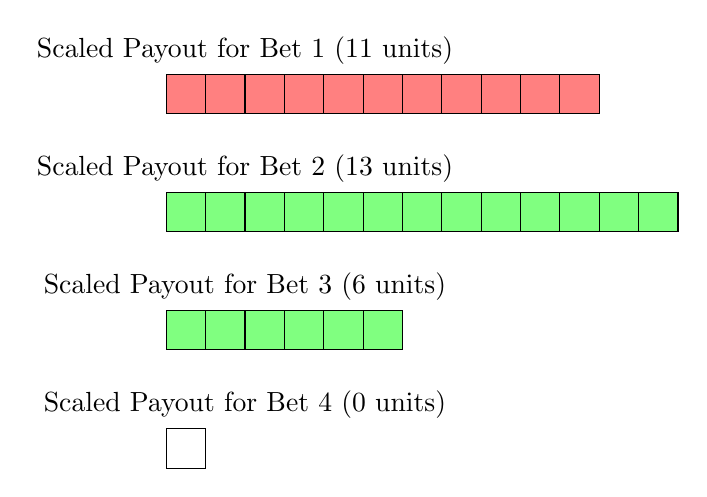
\begin{tikzpicture}[scale=0.5]

% Scaled Payout for Bet 1 (NO)
\foreach \x in {1,...,11}
{
    \draw[fill=red!50] (\x,0) rectangle ++(1,1);
}

% Label for Scaled Payout of Bet 1
\node[above] at (3,1) {Scaled Payout for Bet 1 (\( 11 \text{ units} \))};

% Scaled Payout for Bet 2 (YES)
\foreach \x in {1,...,13}
{
    \draw[fill=green!50] (\x,-3) rectangle ++(1,1);
}

% Label for Scaled Payout of Bet 2
\node[above] at (3,-2) {Scaled Payout for Bet 2 (\( 13 \text{ units} \))};

% Scaled Payout for Bet 3 (YES)
\foreach \x in {1,...,6}
{
    \draw[fill=green!50] (\x,-6) rectangle ++(1,1);
}

% Label for Scaled Payout of Bet 3
\node[above] at (3,-5) {Scaled Payout for Bet 3 (\( 6 \text{ units} \))};

% Scaled Payout for Bet 4 (NO)
\foreach \x in {1,...,1}
{
    \draw[fill=white!50] (\x,-9) rectangle ++(1,1);
}

% Label for Scaled Payout of Bet 4
\node[above] at (3,-8) {Scaled Payout for Bet 4 (\( 0 \text{ units} \))};

\end{tikzpicture}
\end{center}



% Double Divider Line
\begin{center}
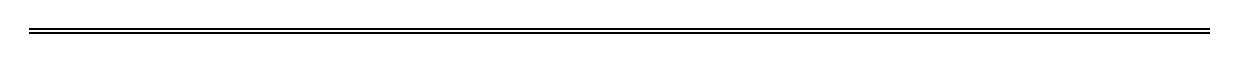
\begin{tikzpicture}[scale=0.5]
\draw[thick] (0,-1) -- (30,-1);
\draw[thick] (0,-1.1) -- (30,-1.1);
\end{tikzpicture}
\end{center}


\end{document}